\section{Data, accounting and calibration}\label{app:database_construction}\label{app:calibration-details}

\subsection{Source coverage and balance-sheet reconciliation}

The Online Appendix explains the public source hierarchy, missing bilateral allocations and the treatment of related offices. The 24-account reporting matrix preserves the rest of the world and unidentified holders and issuers separately. The model groups them into Other counterparties without netting claims; the Eurosystem remains separate. Figure~\ref{fig:full-exposure-network} shows the resulting 22-node network, complementing the bank-focused view in Section~\ref{sec:calibration}. Figure~\ref{fig:active_source_matrix} records source coverage.

\begin{figure}[htbp]
\centering
\floatcaption{Residence-based exposure network, end-2024}{Bk = banks; Gvt = government; NBFI = nonbank financial institutions; Firm = firms; HH = households. Arrows run from creditor to debtor and retain the five largest outgoing claims per node; calculations use the full network. Thickness increases with the claim size in EUR billions. Colours identify countries or aggregate blocks. Gross domestic bank claims are retained in clearing but omitted from this drawing; Figure~\ref{fig:calibrated-exposure-network} displays them as loops.}
\label{fig:full-exposure-network}
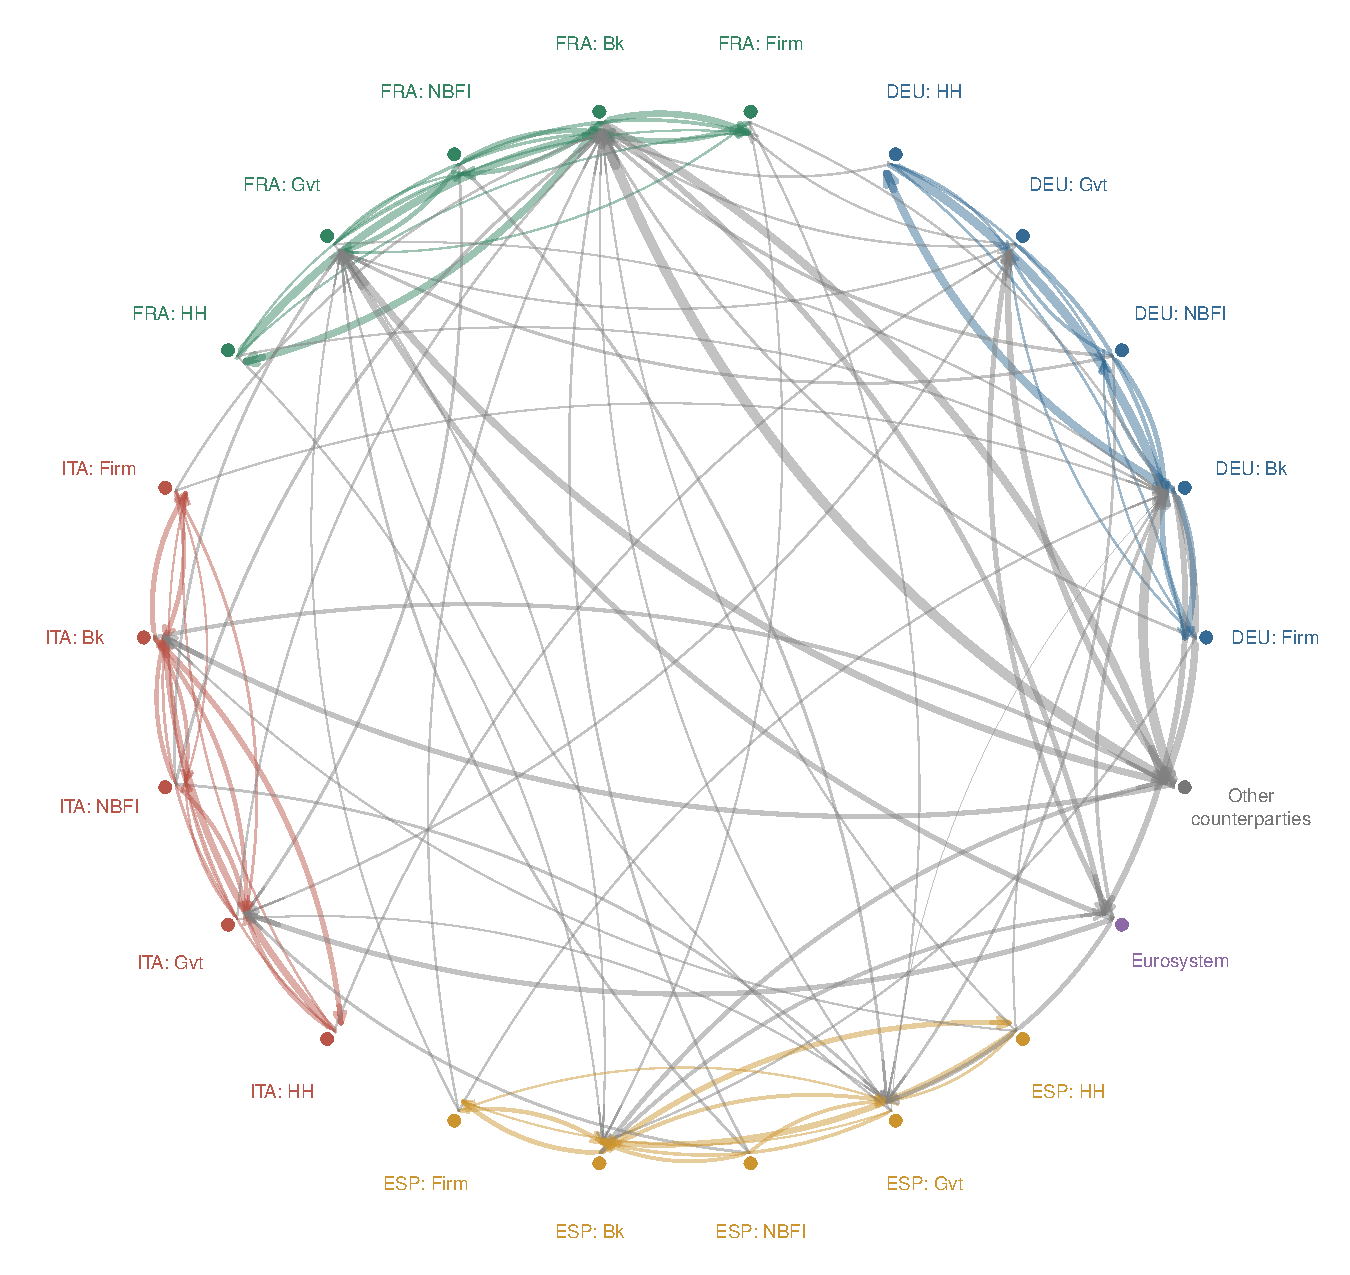
\includegraphics[width=\textwidth]{Figures/figure_network_2024-10-01.pdf}
\end{figure}

\begin{figure}[htbp]
\centering
\floatcaption{Sources represented in the end-2024 residence matrix}{Rows are creditors and columns are debtors. White cells have no positive claim. Cells combining different source layers are marked ``Multiple sources''. Detailed source keys, amounts and reconciliation rules remain in the exposure register.}
\label{fig:active_source_matrix}

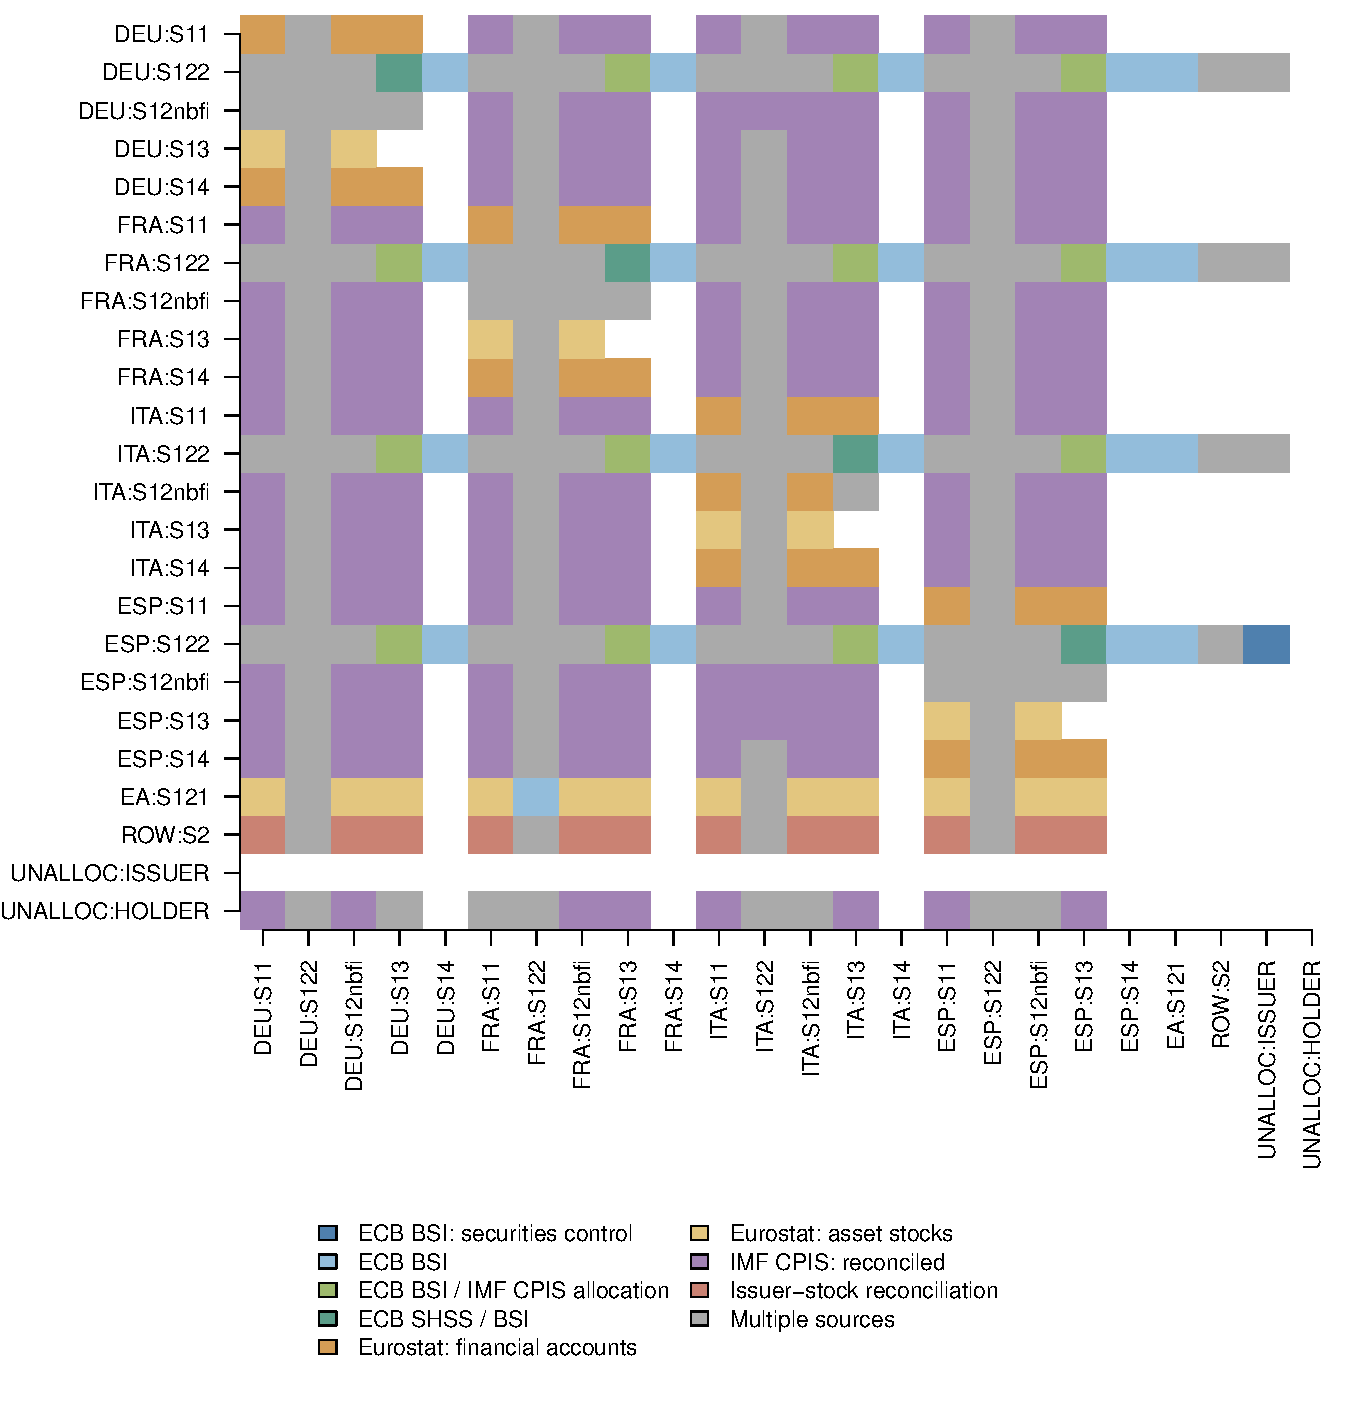
\includegraphics[width=\textwidth]{Figures/active_source_matrix_2024-10-01.pdf}

\end{figure}

The matrix covers selected loans, deposits and debt securities. Other bank assets include government loans, equity holdings, nonfinancial assets and items whose bilateral counterparties are not reconstructed. Coverage and valuation adjustments reconcile these positions to reported balance sheets. Net positions remaining after identified related-office claims are removed are also retained in the reconciliation. These items supply reference repayment resources; they are not independently measured productive wealth.

Write $B_{ij}=x_{ij}$ for banks $i,j$, and $N_{ig}=x_{i,G_g}$ for bank $i$'s holdings of country $g$'s sovereign bonds. Let $D_i^*$ be adjusted statistical liabilities, and let $O_i$ collect net group funding, central-bank funding and remaining or unclassified outside funding settled separately from the common pool. Set
\[
 D_i=D_i^*-O_i,\qquad
 b_i=D_i+E_i-\sum_jB_{ij}-\sum_gN_{ig},
\]
The reference resources therefore satisfy
\[
 b_i+\sum_jB_{ij}+\sum_gN_{ig}=D_i+E_i.
\]
The common pool contains deposits and issued securities. Fixed outside settlements reduce both debt and resources. Provisions against assets are deducted from statistical capital and gross assets together, leaving accounting equity $E_i$. The reference amount $b_i$ includes performing nonbank receipts, outside assets, government loans and coverage or valuation adjustments, net of fixed settlements.

This convention preserves equity but does not assert that the public data identify a single legal recovery class. Remaining liabilities include derivatives and settlement positions, with incomplete public information on close-out rank. The Online Appendix reports the adjustments and statistical-liability benchmarks separately.

\subsection{Prudential headroom and full accounting equity}

For each significant institution, we compute the smaller loss capacity above its published overall risk-weighted capital stack and its leverage requirement. Writing CET1 for Common Equity Tier 1 capital, the country median headroom/CET1 ratio is transferred to resident accounting equity using the same country's public supervisory CET1/equity bridge. Table~\ref{tab:ocr-headroom} reports the resulting headroom and the alternative capacity above a 4.5\% CET1 floor. Consolidated significant institutions and resident offices have different perimeters; these are labelled country proxies, not measured resident regulatory capital.

\begin{table}[htbp]
\centering
\floatcaption{Accounting equity and prudential headroom (EUR billions)}{Equity and clearing debt follow the resident bank balance-sheet reconciliation. OCR headroom uses end-2024 public ECB Pillar 3 and supervisory statistics. ISA headroom is the alternative proxy above a 4.5\% CET1 floor. Neither headroom is substituted for accounting equity in the repayment estate.}
\label{tab:ocr-headroom}
\small

\begin{tabular*}{\textwidth}{@{\extracolsep{\fill}}lrrrr@{}}
\toprule
Country & Accounting equity & Clearing debt & OCR headroom & ISA headroom \\
\midrule
DEU & 686.4 & 7453.6 & 196.8 & 395.5 \\
FRA & 657.0 & 7987.6 & 208.3 & 365.1 \\
ITA & 331.2 & 2697.1 & 90.6 & 168.6 \\
ESP & 245.7 & 2415.9 & 61.5 & 124.5 \\
\bottomrule
\end{tabular*}


\end{table}

Losses exceeding headroom satisfy the first condition for a costly credit event under the disorderly-crisis scenario. An OCR breach can restrict distributions without causing legal default. Market stigma, funding pressure and overlapping constraints can nevertheless impede buffer use \citep{ECBBuffer2023,ECBESRB2026}. The scenario assumes no timely recapitalization or relaxation sufficient to prevent distress. All remaining accounting equity stays in the repayment estate; headroom is never substituted for equity. Partial repayment additionally requires a shortfall after the distress cost.

At the normalized contractual return one, the distress cutoff is $T_i=\min\{D_i+E_i-H_i,D_i/\lambda_i^B\}$. The first term imposes headroom exhaustion; the second ensures that creditors receive less than par on the default branch. Equality gives full repayment. With $H_i=E_i$, the trigger is accounting insolvency; with $\lambda_i^B=1$, the rule becomes ordinary capped pro-rata clearing for any $H_i\leq E_i$.

The baseline $\lambda_i^B=.90$ follows the 10\% remaining-asset default cost in the systemic bank-stress model of \citet{Aikman2009}. It represents realization and franchise disruption in addition to initial credit losses. It is a modelling benchmark, not an estimate of contemporary European administrative resolution costs.

\subsection{Sovereign and private-credit losses}

Safe and contractual bank gross returns equal one. Let $\pi_g^G$ be country $g$'s calibrated annual sovereign-default probability. With 50\% recovery of the contractual payment, sovereign repayments are
\[
 R_g^G(s)=\frac{1-.5\delta_g^G(s)}{1-.5\pi_g^G}.
\]
Mean five-year CDS quotes over December 2007--November 2025 are 14.8, 27.9, 102.5 and 83.9 basis points for Germany, France, Italy and Spain. Let $s_g$ denote these spreads in decimal form. We use them as annual contractual yield-spread proxies, setting $\overline r_g^G=1+s_g$. The expected-payoff normalization $(1-.5\pi_g^G)\overline r_g^G=1$ then gives $\pi_g^G=s_g/[.5(1+s_g)]$, approximately 0.30\%, 0.56\%, 2.03\% and 1.66\%. This is a one-period pricing convention; CDS premium schedules and maturity are not priced separately. These are market-price-based inputs, not historical default frequencies. Marginal risk inputs affect the sovereign payoff normalization; the state comparisons condition on that payoff grid.

The private-credit shock follows the borrower's country. Let $i$ index the creditor's national bank block and $g$ the borrower's country, each among Germany, France, Italy and Spain. The $4\times4$ matrices $\mathbf{F}$ and $\mathbf{Q}$ record bank loans to nonfinancial firms and households, respectively: $F_{ig}$ is the amount lent by banks in country $i$ to firms in country $g$, and $Q_{ig}$ is the corresponding amount lent to households. These loan stocks are extracted from the exposure register; they exclude securities included in the broader sector exposures.

If sovereign $g$ defaults, the scenario imposes an additional loss on those private loans of
\[
 \mathcal L_{ig}=.018F_{ig}+.017Q_{ig}.
\]
For example, a French sovereign default generates private-credit losses for German banks on their loans to French firms and households, even if Germany's sovereign does not default. Summing across borrower countries gives bank $i$'s additional private-credit loss, $\sum_g\mathcal L_{ig}\delta_g^G(s)$, where $\delta_g^G(s)$ equals one if sovereign $g$ defaults in state $s$ and zero otherwise. Its resources before interbank receipts are therefore
\[
 a_i(s)=b_i+\sum_gN_{ig}R_g^G(s)-\sum_g\mathcal L_{ig}\delta_g^G(s).
\]
The sovereign-bond receipts in the second term and the private-loan losses in the third term are distinct channels. The private loss rates, 1.8\% for firm loans and 1.7\% for household loans, are pooled adverse-minus-baseline impairment proxies from the ECB's 2025 bank stress test, Chart 3.8 \citep{ECBStress2025}. Applying them in borrower-country sovereign-default states is a scenario assumption, not an estimated causal relationship. They capitalize a three-year episode once at settlement. Government loans, private securities and outside-sample private loans receive no additional impairment. Opening equity is already net of provisions, so the provision stock is not deducted again. Credit supply and private borrowing remain fixed.

\subsection{NBFI repayment and gross domestic bank claims}

NBFIs have pooled public financial-account buffers and no additional default cost. Financial assets less non-equity liabilities exceed the complete selected bank, NBFI and sovereign claims by approximately EUR~3,500 billion in Germany, 1,329 billion in France, 228 billion in Italy and 377 billion in Spain. With national pooling and other net resources fixed, even zero receipts on these claims leave ordinary debt covered. This establishes par repayment in every equilibrium. An independent eight-node enumeration verifies selected results. Halving NBFI buffer availability also leaves all reported bank equilibrium vectors unchanged.

Identified related-office loans are removed with matched balance-sheet adjustments. The remaining domestic bank claims are retained in $B_{ii}$ as gross obligations among distinct institutions sharing the national repayment rate. The Online Appendix gives a symmetric disaggregation into institutions without own claims that reproduces the block map exactly. It does not rule out asymmetric institutional outcomes. Netting these claims and equal liabilities changes the clearing representation and the estate exposed to costs; this diagnostic removes baseline multiplicity.

\subsection{Weights and comparison with ISA}

Sovereign defaults are independent for the limited set of averages across states reported in the paper; Appendix~\ref{app:ocr_robustness}, Table~\ref{tab:sovereign-dependence}, reports a dependence sensitivity for recovery-backstop averages. In a state with several banking equilibria, the greatest repayment vector receives weight $1-\rho$ and the remaining roots share $\rho$ equally, with $\rho=.20$. A unique root receives weight one. The debt-weighted expected ordinary bank repayment shortfall is approximately 3.0 basis points. State-specific clearing and the maximum capacity over all states do not use these selection weights or the independence convention.

The ECB's Interconnected System-wide stress test Analytics (ISA) application combines granular supervisory and commercial data with liquidity and asset-price feedback \citep{GrassiEtAl2025}. Our public resident-sector network isolates repayment feedback and guarantee capacity. ISA's 4.5\% CET1 default threshold motivates our alternative headroom specification in Appendix~\ref{app:ocr_robustness}, Table~\ref{tab:ocr-robustness} (the row labelled ``ISA headroom''); the baseline uses public OCR/leverage headroom as a conditional distress trigger. The private-credit proxies come from the separate bank stress-test report, not ISA's contagion results. The Online Appendix compares their coverage and thresholds.
